\section{Breadth-first search (BFS) \cite{ai/book/Artificial-Intelligence-A-Modern-Approach/Russell-Norvig}}
\label{AI: Algorithms/Breadth-first search (BFS)}


\begin{figure}[H]
    \centering
    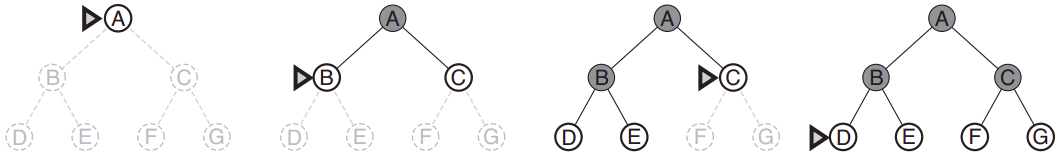
\includegraphics[
        width=\linewidth,
        height=4cm,
        keepaspectratio,
    ]{images/algorithms/Breadth-first-search-BT.png}
    \caption*{
        Breadth-first search on a simple binary tree. At each stage, the node to be expanded next is indicated by a marker.
        \cite{ai/book/Artificial-Intelligence-A-Modern-Approach/Russell-Norvig}
    }
\end{figure}


\begin{enumerate}
    \item Breadth-first search is a simple strategy in which the root node is expanded first, then all the successors of the root node are expanded next, then their successors, and so on. 
    \hfill \cite{ai/book/Artificial-Intelligence-A-Modern-Approach/Russell-Norvig}

    \item In general, all the nodes are expanded at a given depth in the search tree before any nodes at the next level are expanded.
    \hfill \cite{ai/book/Artificial-Intelligence-A-Modern-Approach/Russell-Norvig}

    \item Breadth-first search is an instance of the general graph-search algorithm in which the \textit{shallowest unexpanded node} is chosen for expansion.
    \hfill \cite{ai/book/Artificial-Intelligence-A-Modern-Approach/Russell-Norvig}

    \item new nodes (which are always deeper than their parents) go to the back of the queue, and old nodes, which are shallower than the new nodes, get expanded first. 
    \hfill \cite{ai/book/Artificial-Intelligence-A-Modern-Approach/Russell-Norvig}

    \item There is one slight tweak on the general graph-search algorithm, which is that the goal test is applied to each node when it is generated rather than when it is selected for expansion.
    \hfill \cite{ai/book/Artificial-Intelligence-A-Modern-Approach/Russell-Norvig}
    \\
    If the algorithm were to apply the goal test to nodes when selected for expansion, rather than when generated, the whole layer of nodes at depth d would be expanded before the goal was detected and the time complexity would be $\mathcal{O}(b\ ^{d+1})$.
    \hfill \cite{ai/book/Artificial-Intelligence-A-Modern-Approach/Russell-Norvig}

    \item the algorithm, following the general template for graph search, discards any new path to a state already in the frontier or explored set; it is easy to see that any such path must be at least as deep as the one already found. 
    \hfill \cite{ai/book/Artificial-Intelligence-A-Modern-Approach/Russell-Norvig}

    \item breadth-first search \textbf{always} has the \textit{shallowest path} to every node on the frontier. 
    As soon as a goal node is generated, we know it is the shallowest goal node because all shallower nodes must have been generated already and failed the goal test. 
    \hfill \cite{ai/book/Artificial-Intelligence-A-Modern-Approach/Russell-Norvig}

    \item \textbf{performance}:
    \begin{enumerate}
        \item \textbf{complete}: if the shallowest goal node is at some finite depth $d$, breadth-first search will eventually find it after generating all shallower nodes (provided the branching factor $b$ is finite). 
        \hfill \cite{ai/book/Artificial-Intelligence-A-Modern-Approach/Russell-Norvig}

        \item  the shallowest goal node is \textbf{not necessarily} the \textit{optimal} one. 
        breadth-first search is optimal if the path cost is a non-decreasing function of the depth of the node.
        The most common such scenario is that all actions have the same cost.
        the algorithm is optimal if step costs are all identical.
        \hfill \cite{ai/book/Artificial-Intelligence-A-Modern-Approach/Russell-Norvig}

        \item \textbf{Space Complexity}:
        \begin{enumerate}
            \item explored set: $\mathcal{O}(b\ ^{d-1})$
            \hfill \cite{ai/book/Artificial-Intelligence-A-Modern-Approach/Russell-Norvig}

            \item frontier: $\mathcal{O}(b\ ^{d})$
            \hfill \cite{ai/book/Artificial-Intelligence-A-Modern-Approach/Russell-Norvig}

            \item overall: $\mathcal{O}(b\ ^{d})$
            \hfill \cite{ai/book/Artificial-Intelligence-A-Modern-Approach/Russell-Norvig}
        \end{enumerate}

        \item \textbf{Time Complexity}: 
        $\mathcal{O}(b\ ^{d})$
        \hfill \cite{ai/book/Artificial-Intelligence-A-Modern-Approach/Russell-Norvig}

    \end{enumerate}

    \item \textbf{Disadvantages}:
    \begin{enumerate}
        \item the memory requirements are a bigger problem for breadth-first search than is the execution time.
        \hfill \cite{ai/book/Artificial-Intelligence-A-Modern-Approach/Russell-Norvig}

        
    \end{enumerate}

\end{enumerate}


\subsection*{Implementation}

\begin{enumerate}
    \item \textbf{frontier}: FIFO queue
\end{enumerate}


\vspace{0.5cm}


\begin{algorithm}[H]
    \caption{Breadth-first search on a graph. \cite{ai/book/Artificial-Intelligence-A-Modern-Approach/Russell-Norvig}}

    \SetKwFunction{FUNCTION}{\textsc{Breadth-First-Search}}
    \SetKwProg{Fn}{function}{ returns \normalfont{a solution, or failure}}{end}
    \Fn{\FUNCTION{problem}}{
        $node \ \gets$ a node with \textsc{State} = $problem$.\textsc{Initial-State}, \textsc{Path-Cost} = $0$ \\
        \lIf{$problem$.\textsc{Goal-Test}($node$.\textsc{State})}{
            \Return \textsc{Solution}($node$)
        }
        $frontier \ \gets$ a FIFO queue with node as the only element \\
        $explored \ \gets$ an empty set \\
        \ \\
        \While{}{
            \lIf{\textsc{Empty?}($frontier$)}{
                \Return failure
            }
            \Comment{chooses the shallowest node in $frontier$}
            $node \ \gets$ \textsc{Pop}($frontier$) \\ 
            add $node$.\textsc{State} to $explored$ \\
            \ \\
            \ForEach{$action$ \textbf{in} $problem$.\textsc{Actions}($node$.\textsc{State})}{
                $child \gets$ \textsc{Child-Node}($problem,\ node,\ action$) \\
                \If{$child$.\textsc{State} is \textbf{not in} $explored$ or $frontier$}{
                    \lIf{$problem$.\textsc{Goal-Test}($child$.\textsc{State})}{
                        \Return \textsc{Solution}($child$)
                    }
                    $frontier \gets$ \textsc{Insert}($child,\ frontier$)
                }
            }
        }
    }
\end{algorithm}


\begin{lstlisting}[
    language=Python,
    caption=Problem Solving Agent - Breadth-first search on a graph
]
from queue import Queue

def breadth_first_search(problem: Problem):
    node = Node(problem.initial_state, None, None, 0)

    if problem.goal_test(node.state):
        return solution(node)
    
    frontier = Queue()
    explored = set()

    frontier.put(node)

    while True:
        if frontier.empty():
            return None
        
        node = frontier.get()
        explored.add(node)

        for action in problem.actions(node.state):
            child = child_node(problem, node, action)
            
            if (not any([n.state == child.state for n in frontier.queue]) and 
                not any([n.state == child.state for n in explored])):
                if problem.goal_test(child.state):            
                    return solution(child)

                frontier.put(child)
\end{lstlisting}











